\let\negmedspace\undefined
\let\negthickspace\undefined
\documentclass[journal]{IEEEtran}
\usepackage[a5paper, margin=10mm, onecolumn]{geometry}
%\usepackage{lmodern} % Ensure lmodern is loaded for pdflatex
\usepackage{tfrupee} % Include tfrupee package

\setlength{\headheight}{1cm} % Set the height of the header box
\setlength{\headsep}{0mm}     % Set the distance between the header box and the top of the text

\usepackage{gvv-book}
\usepackage{gvv}
\usepackage{cite}
\usepackage{amsmath,amssymb,amsfonts,amsthm}
\usepackage{algorithmic}
\usepackage{graphicx}
\usepackage{textcomp}
\usepackage{xcolor}
\usepackage{txfonts}
\usepackage{listings}
\usepackage{enumitem}
\usepackage{mathtools}
\usepackage{gensymb}
\usepackage{comment}
\usepackage[breaklinks=true]{hyperref}
\usepackage{tkz-euclide} 
\usepackage{listings}
% \usepackage{gvv}                               

\def\inputGnumericTable{}                      
\usepackage[latin1]{inputenc}                    
\usepackage{color}                              
\usepackage{array}                             
\usepackage{longtable}                          
\usepackage{calc}                               
\usepackage{multirow}                           
\usepackage{hhline}                            
\usepackage{ifthen}                          
\usepackage{lscape}
\begin{document}

\bibliographystyle{IEEEtran}
\vspace{3cm}

\title{1.7.10}
\author{AI25BTECH11024 - Pratyush Panda
}
\maketitle
% \newpage
% \bigskip
{\let\newpage\relax\maketitle}

\renewcommand{\thefigure}{\theenumi}
\renewcommand{\thetable}{\theenumi}
\setlength{\intextsep}{10pt} % Space between text and floats


\numberwithin{equation}{enumi}
\numberwithin{figure}{enumi}
\renewcommand{\thetable}{\theenumi}

\textbf{Question: }\\
Find the relation between $x$ and $y$ if the points $\Vec{A}(x, y)$, $\Vec{B}(-5, 7)$ and $\Vec{C}(-4, 5)$ are collinear.

\textbf{Solution: } \\
Given:
$$
\Vec{A}=\myvec{x \\ y} ; \Vec{B}=\myvec{-5 \\ 7} ; \Vec{C}=\myvec{-4 \\ 5}
$$

Now we have to form the Matrix,\\
\begin{align}
\Vec{M}=\myvec{A-C & B-C}^T
\end{align}
\begin{align}
\Vec{M}=\myvec{x+4 & y-5 \\ -1 & 2}
\end{align}

Now to get the RREF of this Matrix we can apply the following row operations:
\begin{align}
\myvec{x+4 & y-5 \\ -1 & 2} \xrightarrow{R_2 \longleftrightarrow R_2 + \frac{1}{x+4}R_1} \myvec{x+4 & y-5 \\ 0 & 2 + \frac{y-5}{x+4}}
\end{align}

For this matrix to have $rank=1$, the second element of the second row should also be $0$

Therefore, we get
\begin{align}
2 + \frac{y-5}{x+4} = 0
\end{align}

On simplifying,
\begin{align}
y = -2x -3
\end{align}

\begin{figure}[H]
\centering
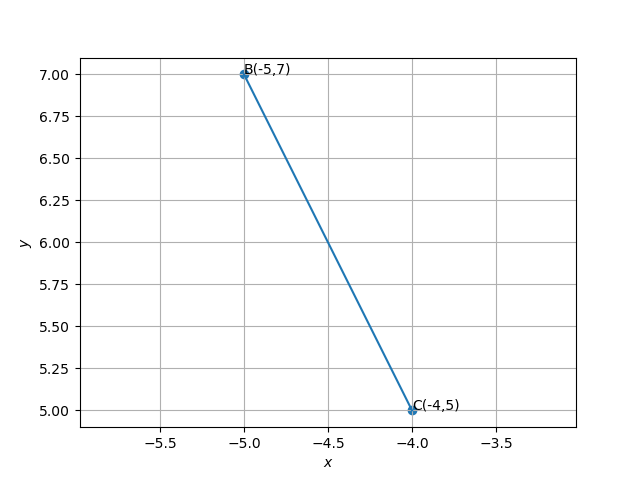
\includegraphics[width=0.6\columnwidth]{figs/img.png}
\caption*{}
\end{figure}

\end{document}
